% This is samplepaper.tex, a sample chapter demonstrating the
% LLNCS macro package for Springer Computer Science proceedings;
% Version 2.21 of 2022/01/12
%
\documentclass[runningheads]{llncs}
%
\usepackage[T1]{fontenc}
% T1 fonts will be used to generate the final print and online PDFs,
% so please use T1 fonts in your manuscript whenever possible.
% Other font encondings may result in incorrect characters.
%
\usepackage[utf8]{inputenc}
\usepackage[english]{babel}
\usepackage{booktabs}
\usepackage{hyperref}
\usepackage{graphicx}
% Used for displaying a sample figure. If possible, figure files should
% be included in EPS format.
%
\usepackage[vlined,algoruled,linesnumbered]{algorithm2e}
\usepackage{amsmath,amssymb,nccmath,mathtools,stmaryrd}
\usepackage{tabularx}
\usepackage{multicol}
\usepackage{siunitx}
% If you use the hyperref package, please uncomment the following two lines
% to display URLs in blue roman font according to Springer's eBook style:
\usepackage{xcolor}
\renewcommand\UrlFont{\color{blue}\rmfamily}
\urlstyle{rm}
%
\begin{document}
%
\title{Masked Computation of the Floor Function and Its Application to the FALCON Signature}
%
\titlerunning{Masked Floor Function For FALCON}
% If the paper title is too long for the running head, you can set
% an abbreviated paper title here
%
\author{Justine Paillet\inst{1,3}\orcidID{0009-0009-6056-7766} \and
  Pierre-Augustin Berthet\inst{2,3}\orcidID{0009-0005-5065-2730} \and
C\'edric Tavernier\inst{3}\orcidID{0009-0007-5224-492X}}
%
\authorrunning{J. Paillet et al.}
% First names are abbreviated in the running head.
% If there are more than two authors, 'et al.' is used.
%
\institute{
  Université Jean-Monnet, Saint-\'Etienne, France, \email{justine.paillet@univ-st-etienne.fr}
  \and
  Télécom Paris, Palaiseau, France, \email{berthet@telecom-paris.fr}
  \and
  Hensoldt SAS FRANCE, Plaisir, France, \email{<pierre-augustin.berthet,justine.paillet,cedric.tavernier>@hensoldt.net}
}
%
\maketitle              % typeset the header of the contribution
%
\begin{abstract}
With the ongoing standardization of new Post Quantum Cryptography (PQC) primitives by the National Institute of Standards and Technology (NIST), it is important to investigate the robustness of new designs to Side Channel Analysis (SCA). Amongst those future standards is Falcon, a lattice-based signature which relies of rational numbers. It thus requires an implementation using floating point arithmetic, which is harder to design well and secure. While recent work proposed a solution to mask the addition and the multiplication, some roadblocks remains, most noticeably how to protect the floor function. In this work we propose several methods to protect the computation of the floor function. We provide mathematical proofs of our methods as well as formal security proof in the probing model using the Non-Interference concepts. We also discuss their application to the FALCON Signature.

\keywords{Floor Function \and Floating-Point Arithmetic \and Post-Quantum Cryptography \and FALCON \and Side-Channel Analysis \and Masking}
\end{abstract}
%
%
%
\section{Notations}
\subsection{Diagram Legend}
\cite{10.1007/3-540-68697-5_9}
The following diagrams (\emph listofalldiagram figures) use the same legend:\begin{itemize}
    \item Probing sets are denoted by $P_i$ or $O$ and are colored in \textcolor{red}{red}.
    \item Simulation sets are denoted by $S_i^j$ and are colored in \textcolor{blue}{blue}.
    \item \emph{t-SNI} gadgets are colored in \textcolor{green}{green}.
    \item \emph{t-NI} gadgets are colored in \textcolor{black}{black}.
\end{itemize}
\section{Proofs}
\subsection{SetExZero}
\label{alg:setexzero}
\begin{figure}[!ht]
    \centering
    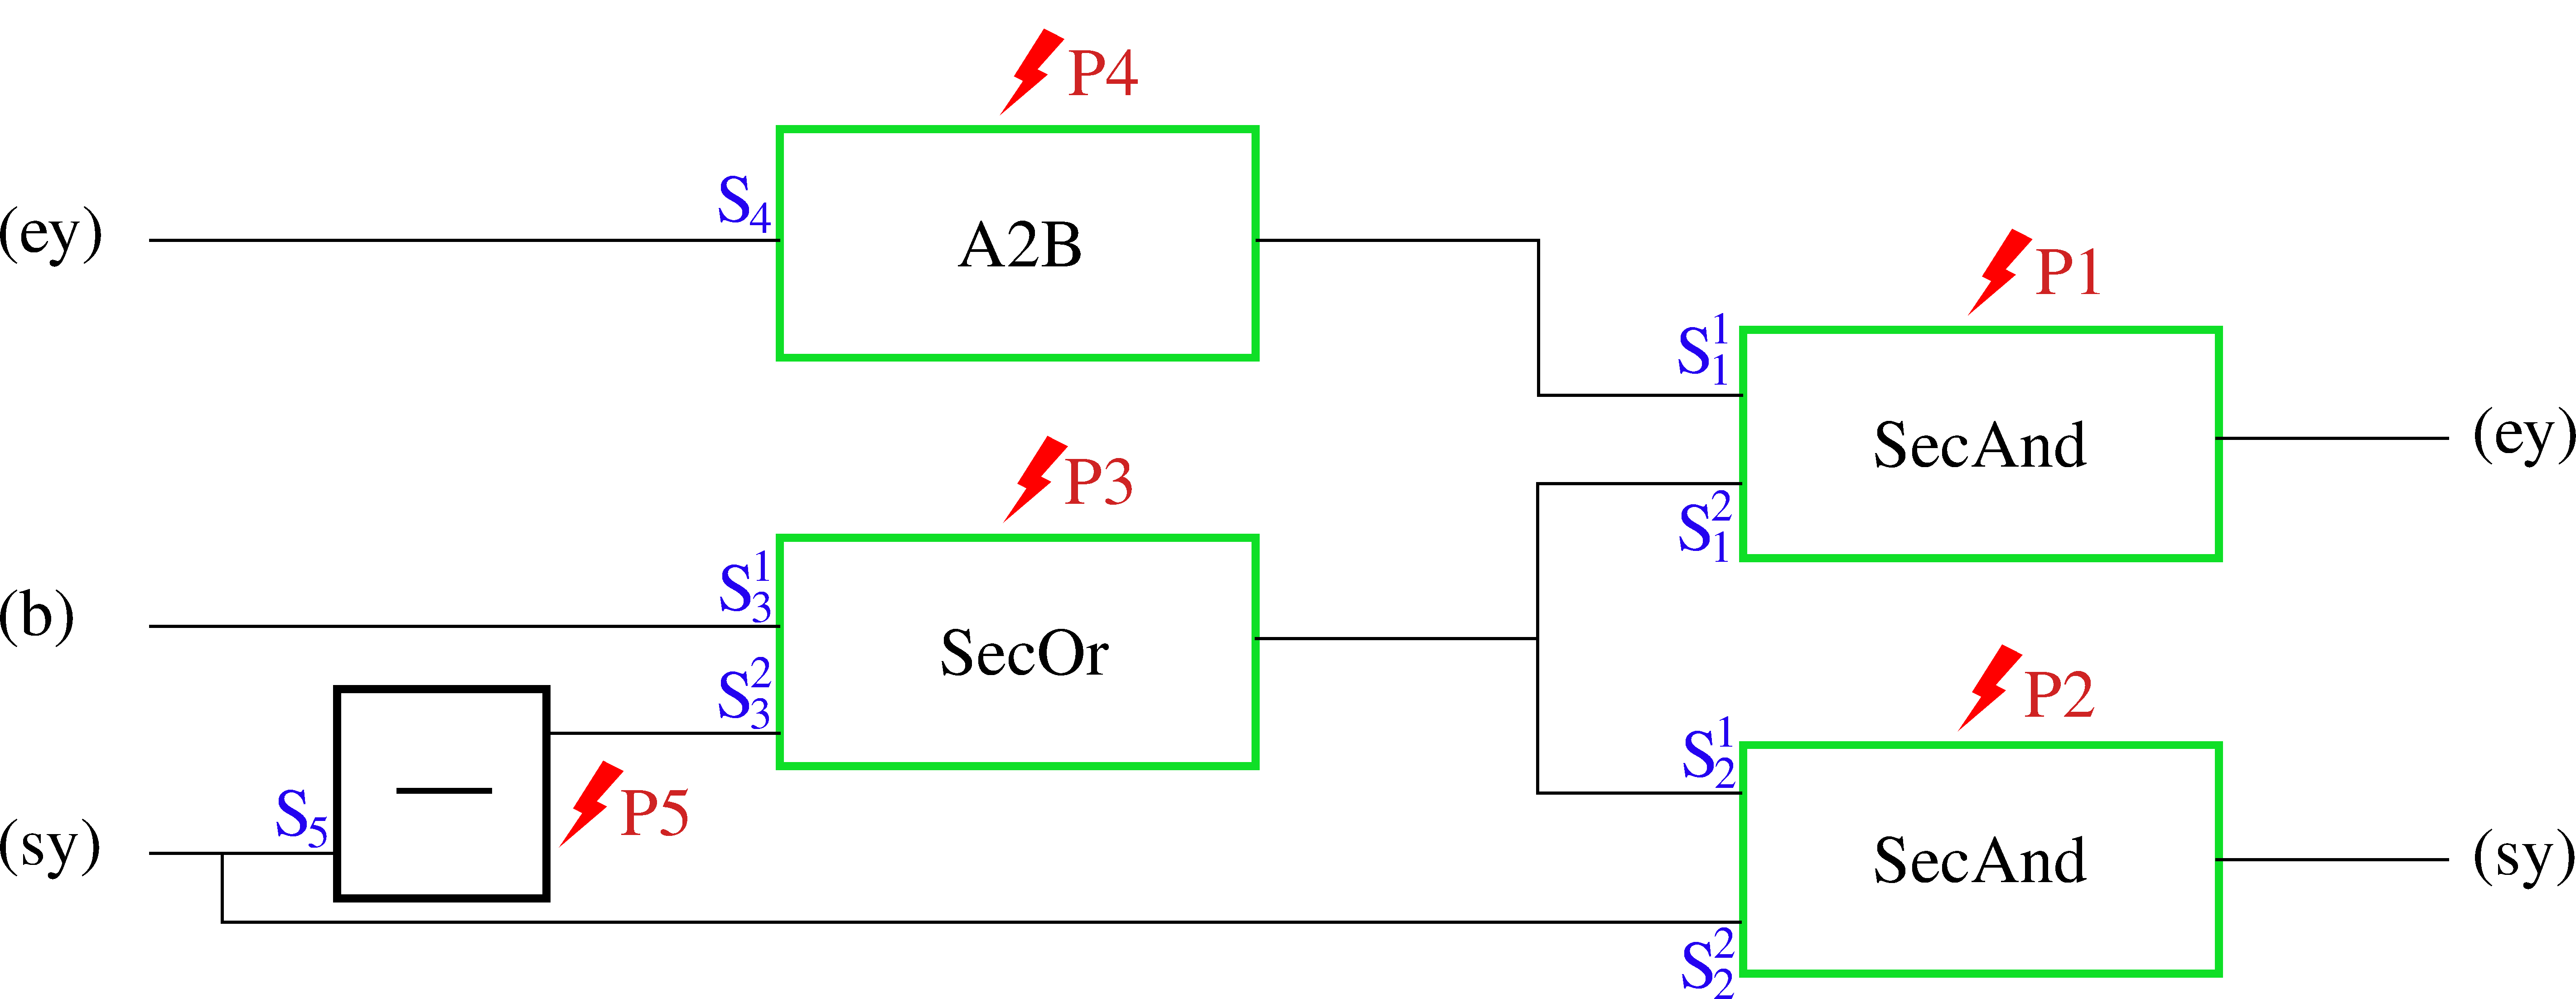
\includegraphics[width=7cm]{figure/SetExZero.pdf}
    \caption{Abstract diagram of Gadget \emph{SetExZero}}
    \label{fig:setexzero}
\end{figure}
\begin{lemma}\label{lem:setexzero}
    The gadget \emph{SetExZero} (Algorithm \ref{alg:setexzero}) is \emph{t-SNI} secure.    
\end{lemma}
\begin{proof}\label{proof:setexzero}
    We use an abstract diagram in Figure \ref{fig:setexzero} to demonstrate our proof. Let assume an adversary probes $t$ values, including the probing sets $P_i$ for $i\in\llbracket 1;5\rrbracket$. Let assume the simulation sets $S_i^j$ for some $j$ necessary to simulate the corresponding gadgets. \emph{t-SNI} security implies that if the size of all probing sets $P_i$ is $t_I\leq t$ and if the size of values required to simulate in each gadget is smaller than $t$, then the simulation sets linked to the input shares are not bigger than $t_I$.\newline
    \emph{SecAnd},\emph{SecOr} and \emph{A2B} being \emph{t-SNI} gagdets, we have the following:
    \begin{multicols}{2}
        \begin{itemize}
            \item $|S_1^1|,|S_1^2|\leq|P_1|$
            \item $|S_2^1|,|S_2^2|\leq|P_2|$
            \item $|S_3^1|,|S_3^2|\leq|P_3|$
            \item $|S_4|\leq|P_4|$
        \end{itemize}
    \end{multicols}
    Finally, \emph{-} being \emph{t-NI}, $|S_5|\leq|P_5|+|S_3^2|\leq|P_5|+|P_3|$. Based on the previous inequalities, one can check that no gadget requires more than $t_i$ values to be simulated. Finally, we can use at most $|S_4|\leq|P_4|$ shares of $ey$, $|S_3^1|\leq|P_3|$ shares of $b$ and $|S_5 \cup S_2^2| \leq |P_5| + |P_3| + |P_2|$ shares of $sy$ to simulate all the probed values, none being more than $t_I$.
\end{proof}

\subsection{SecFprUrshMod}
\label{alg:secfprurshmod}
\begin{figure}[!ht]
    \centering
    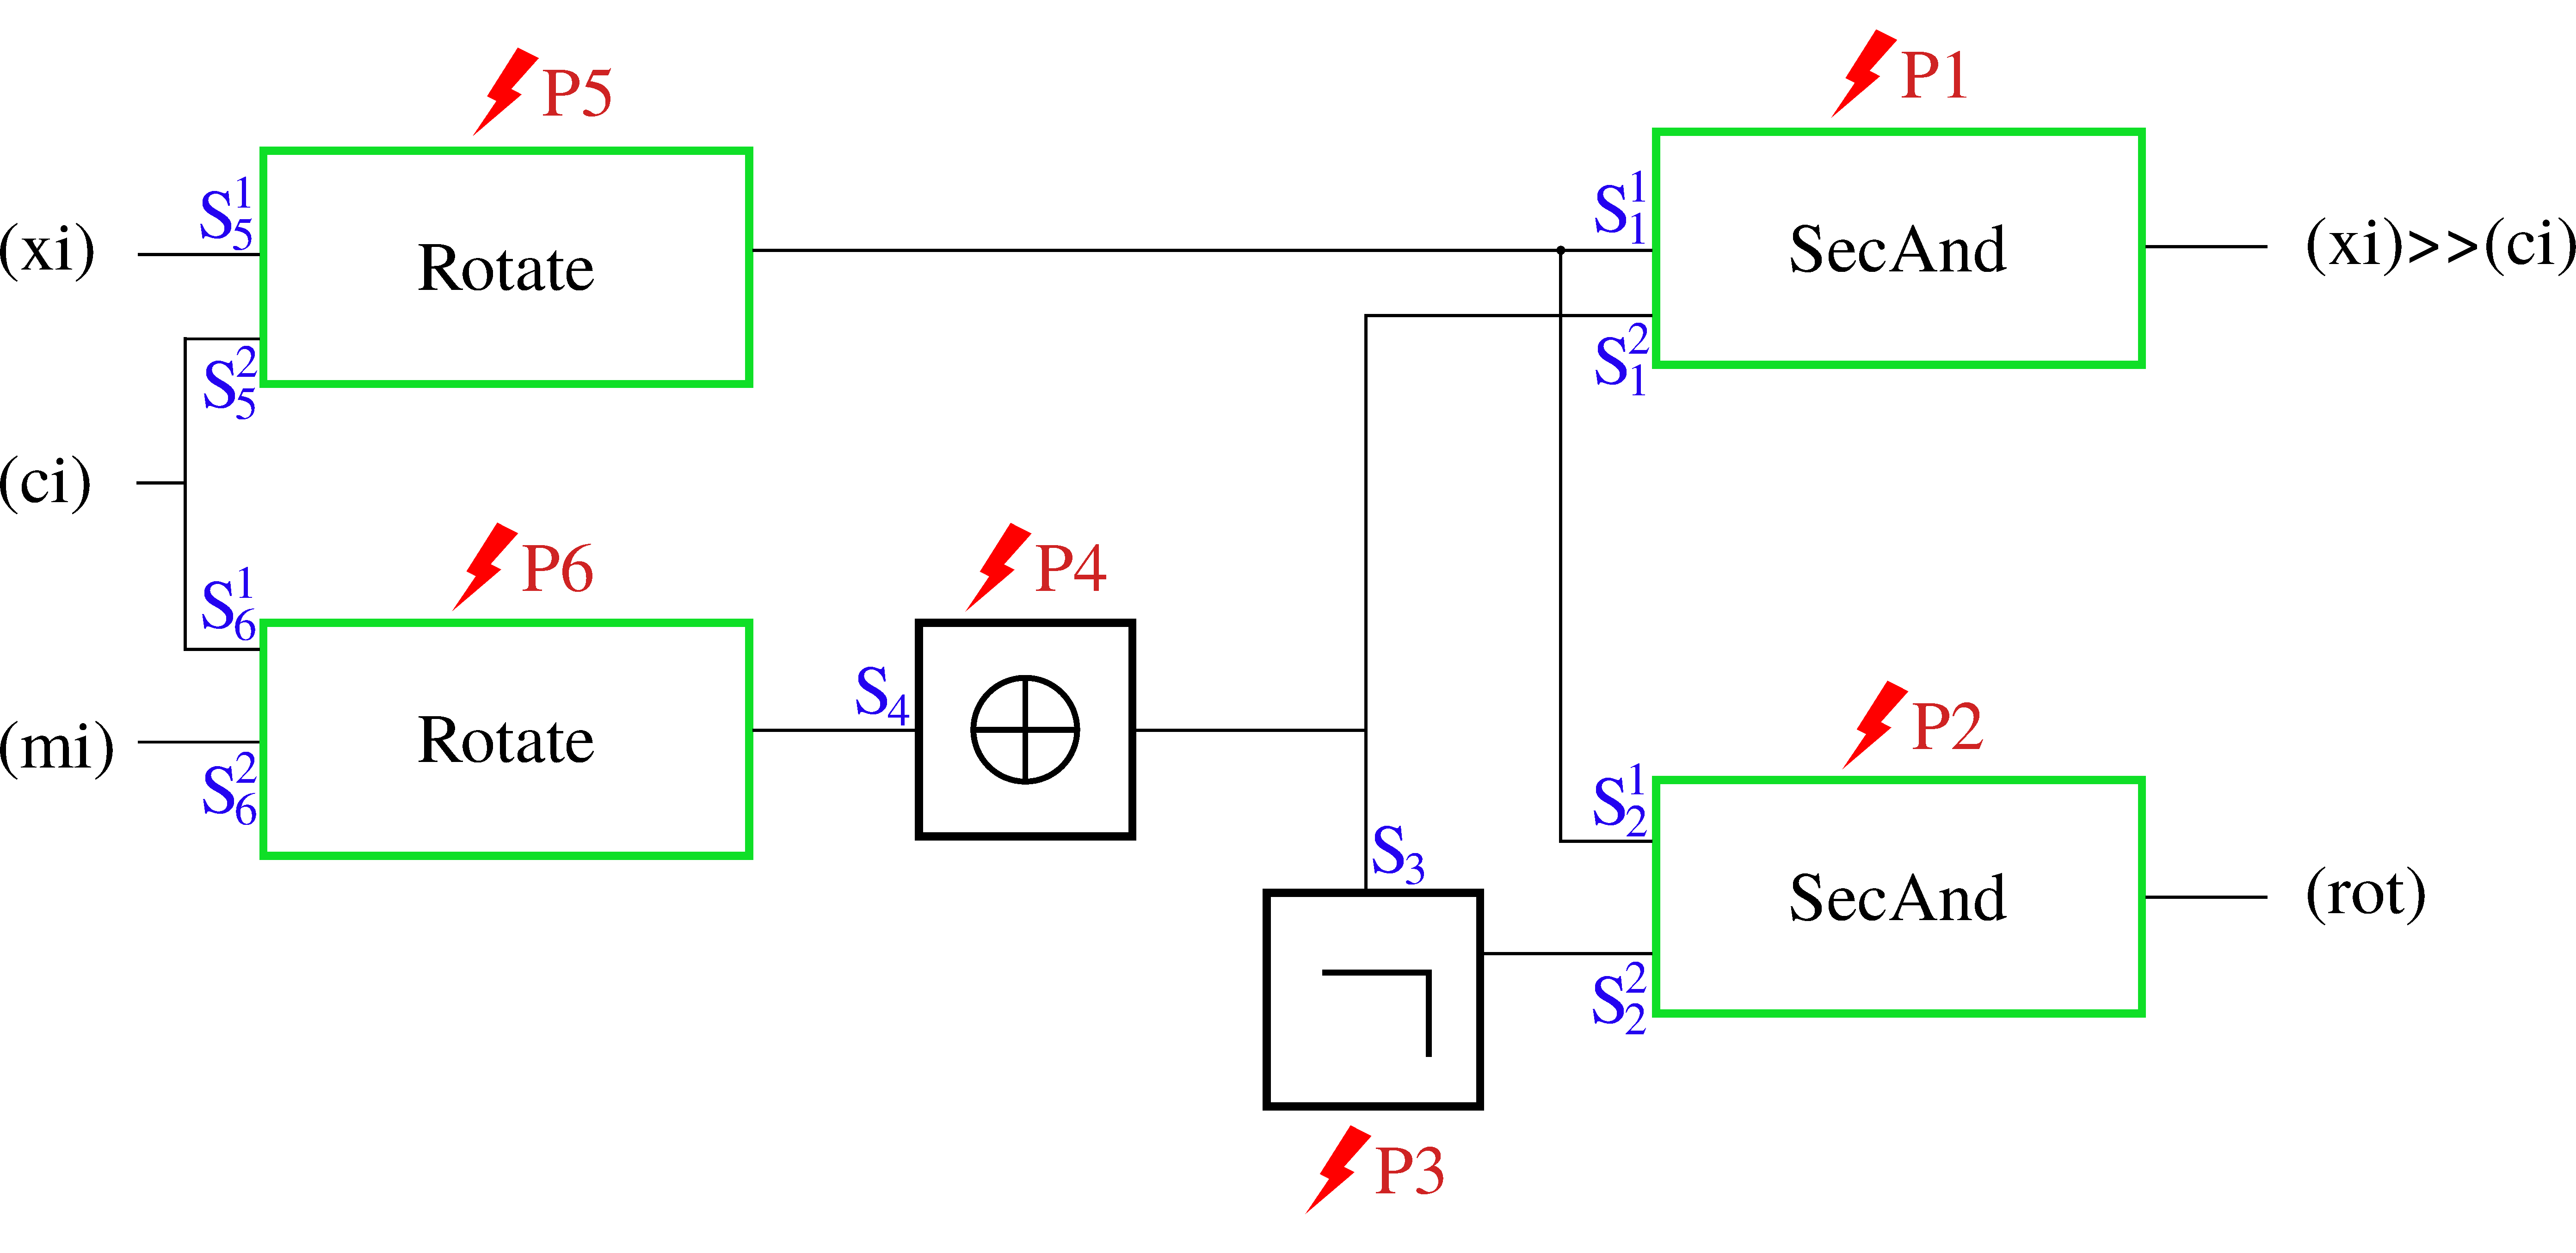
\includegraphics[width = 7cm]{figure/secfprurshmod.pdf}
    \caption{Abstract diagram for gadget \emph{SecFprUrshMod}}
    \label{fig:secfprurshmod}
\end{figure}
\begin{lemma}\label{lem:secfprurshmod}
    The gadget \emph{SecFprUrshMod} (Algorithm \ref{alg:secfprurshmod}) is \emph{t-SNI} secure.    
\end{lemma}
\begin{proof}
    We will make the same assumptions as in Proof \ref{proof:setexzero}. We rely on an abstract diagram of \emph{SecFprUrshMod} in Figure \ref{fig:secfprurshmod} to demonstrate our lemma. As the input shares are immediately fed into \emph{t-SNI} gadgets, we will check if the \emph{t-SNI} security holds for internal states of the algorithm. We have the following inequalities:
    \begin{multicols}{2}
        \begin{itemize}
            \item $|S_1^1|,|S_1^2|\leq|P_1|$
            \item $|S_2^1|,|S_2^2|\leq|P_2|$
            \item $|S_3|\leq|P_3| + |S_2^2| \leq |P_3| + |P_2|$
            \item $|S_4|\leq|P_4| + |S_3| + |S_1^2| \leq |P_4| + |P_3| + |P_2| + |P_1|$
            \item $|S_5^1|,|S_5^2| \leq |P_5|$
            \item $|S_6^1|,|S_6^2| \leq |P_6|$
        \end{itemize}
    \end{multicols}
    The number of values to simulate in each gadget is no more than $t_I$. This also applies to the input shares, with $|S_5^1| \leq |P_5|$ for $xi$, $|S_5^2 \cup S_6^1| \leq |P_5| + |P_6|$ for $ci$ and $|S_6^2| \leq |P_6|$ for $mi$.
\end{proof}

\subsection{RemoveDecimal}
\label{alg:removedecimal}
\begin{figure}[!ht]
    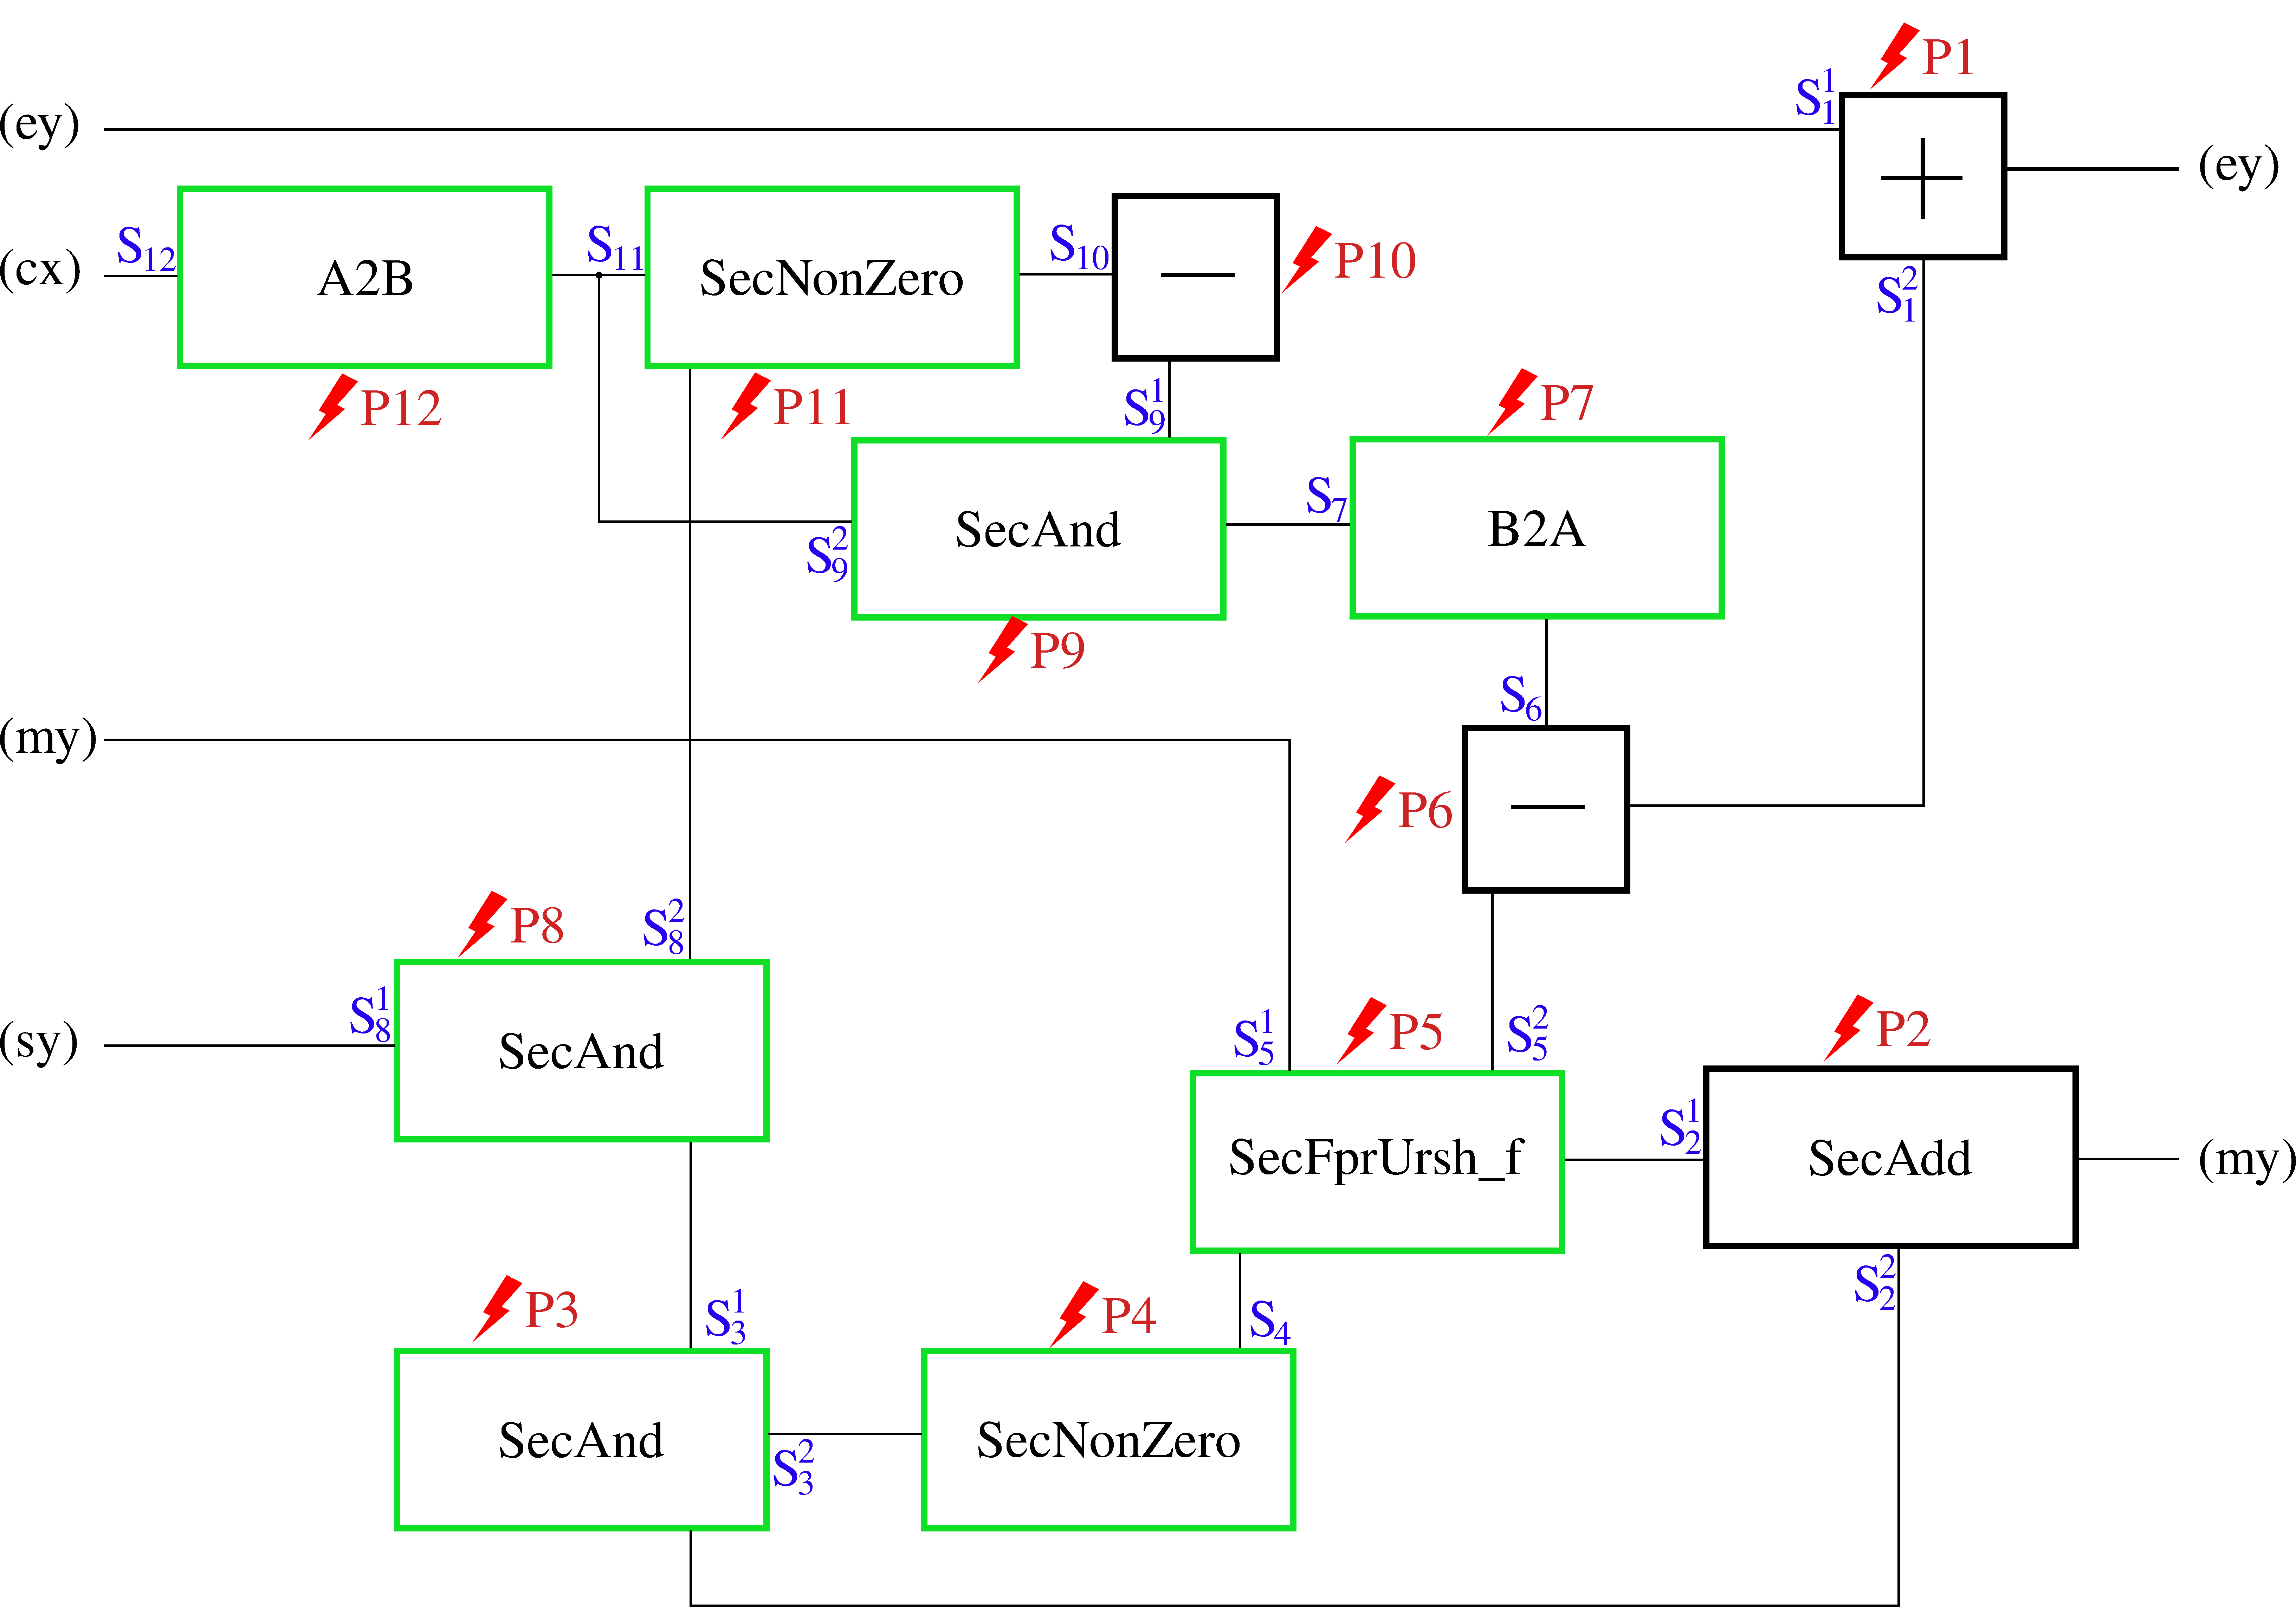
\includegraphics[width=7cm]{figure/RemoveDec.pdf}
    \caption{Abstract diagram for gadget \emph{RemoveDecimal}}
    \label{fig:removedecimal}
\end{figure}
\begin{lemma}\label{lem:removedecimal}
    The gadget \emph{RemoveDecimal} (Algorithm \ref{alg:removedecimal}) is \emph{t-SNI} secure.    
\end{lemma}
\begin{proof}
    We will make the same assumptions as in Proof \ref{proof:setexzero}. We use an abstract diagram of \emph{RemoveDecimal} in Figure \ref{fig:removedecimal} to demonstrate our lemma. We have the following inequalities:
    \begin{multicols}{2}
        \begin{itemize}
            \item $|S_1^1|,|S_1^2|\leq|P_1| + |O_{ey}|$
            \item $|S_2^1|,|S_2^2|\leq|P_2| + |O_{my}|$
            \item $|S_3|\leq |P_3|$
            \item $|S_4|\leq|P_4|$
            \item $|S_5^1|,|S_5^2| \leq |P_5|$
            \item $|S_6| \leq |P_6| + |S_1^2| \leq |P_6| + |P_1| + |O_{ey}|$
            \item $|S_7|\leq|P_7|$
            \item $|S_8^1|,|S_8^2|\leq|P_8|$
            \item $|S_9^1|,|S_9^2| \leq|P_9|$
            \item $|S_10|\leq|P_10| + |S_9^1| \leq |P_10| + |P_9|$
            \item $|S_11| \leq |P_11|$
            \item $|S_12| \leq |P_12|$
            \item $|S_13| \leq |P_13|$
        \end{itemize}
    \end{multicols}

\end{proof}

\subsection{SecBaseInt}
\label{alg:secbaseint}
\begin{figure}[!ht]
    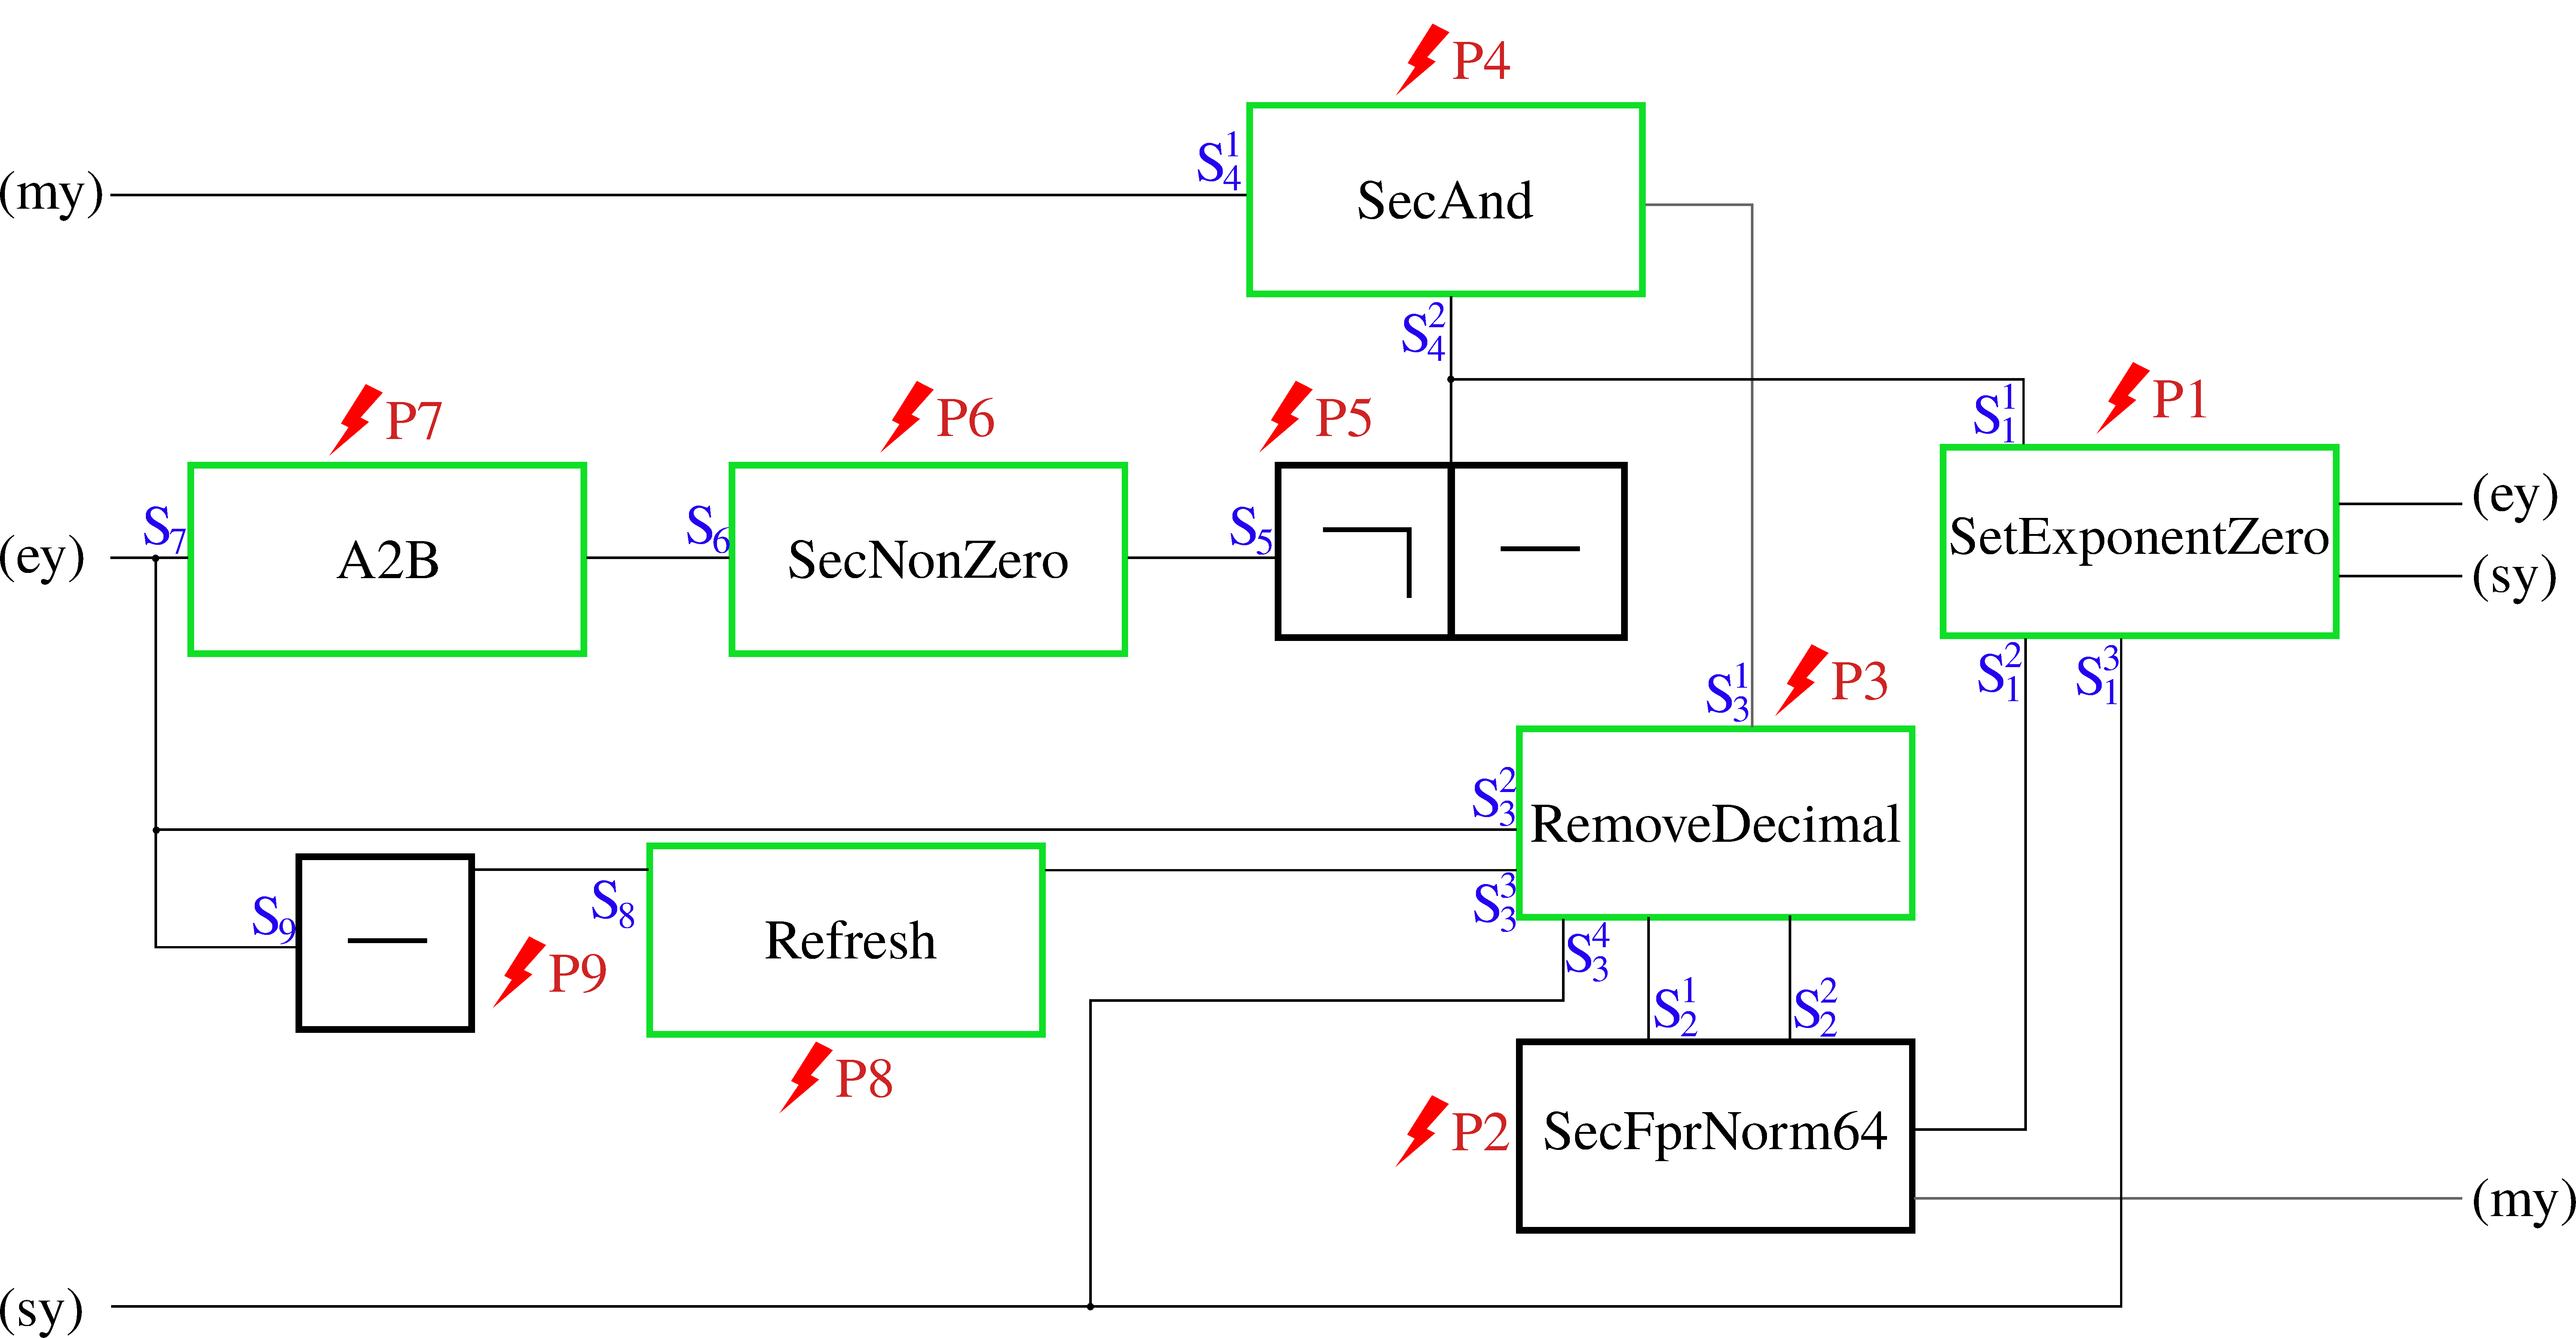
\includegraphics[width=7cm]{figure/secbaseint.pdf}
    \caption{Abstract diagram for gadget \emph{SecBaseInt}}
    \label{fig:secbaseint}
\end{figure}
\begin{lemma}\label{lem:secbaseint}
    The gadget \emph{SecBaseInt} (Algorithm \ref{alg:secbaseint}) is \emph{t-SNI} secure.    
\end{lemma}
\begin{proof}
    We will make the same assumptions as in Proof \ref{proof:setexzero}. We use an abstract diagram of \emph{SecBaseInt} in Figure \ref{fig:secbaseint} to demonstrate our lemma. We have the following inequalities:
    \begin{multicols}{2}
        \begin{itemize}
            \item $|S_1^1|,|S_1^2|,|S_1^3|\leq|P_1|$
            \item $|S_2^1|,|S_2^2|\leq|P_2| + |O_{my}|$
            \item $|S_3^1|,|S_3^2|, |S_3^3|, |S_3^4| \leq|P_3|$
            \item $|S_4^1|,|S_4^2|\leq|P_4|$
            \item $|S_5| \leq |P_5|$
            \item $|S_6| \leq |P_6|$
            \item $|S_7| \leq |P_7|$
            \item $|S_8| \leq |P_8|$
            \item $|S_9| \leq |P_9| + |S_8| \leq |P_9| + |P_8|$
        \end{itemize}
    \end{multicols}
    The number of values to simulate in each gadget is no more than $t_I$. This also applies to the input shares, with $|S_4^1| \leq |P_4|$ for $my$, $|S_7 \cup S_3^2 \cup S_9| \leq |P_7| + |P_3| + |P_9| + |P_8|$ for $ey$ and $|S_3^4 \cup S_1^3| \leq |P_3| + |P_1|$ for $sy$.
\end{proof}

\begin{algorithm}
    \caption{SecFprBaseInt(x, f)}
    \label{algo:SecFprBaseInt}
    \KwData{64-bit boolean shares $(x_i)_{1\leq i \leq n}$ for value x \\
    A function f : floor, round or trunc.}
    \KwResult{64-bit boolean shares $(y_i)_{1\leq i \leq n}$ for mantissa value y = floor(x)/round(x)/trunc(x).} 
    $((my_i), (ey_i), (sy_i)) \leftarrow$ SecFprExtract($(x_i)$)\;%\tcp*{extract mantissa, exponent and sign}
    $(cx_i) \leftarrow (ey_i)$\;
    $cx_1 \leftarrow ey_1 - \text{Zero}_f$\;%\tcp*{$\text{Zero}_f$ = 1023 for floor }%and trunc, $\text{Zero}_f$ = 1022 for round}
    $(c_i) \leftarrow$ A2B($(cx_i^{(16)})$)\; 
    $(c_i) \leftarrow$ SecNonZero($(c_i)$)\tcp*{check if the exponent is negative}
    $(b_i) \leftarrow (\neg(-c_i))$\;
    Refresh($(cx_i)$)\;
    $(my_i) \leftarrow$ SecAnd($(my_i), (b_i)$)\;%\tcp*{if c = 0,  my = mx and if c = 1, my = 0 }
    $(my_i), (ey_i), (Rnd_i) \leftarrow$ RemoveDecimal$_f((my_i), (ey_i), (sy_i), (cx_i)$)\;% \tcp*{depends on f}
    $(my_i), (ey_i) \leftarrow$ SecFprNorm64($(my_i),(ey_i)$)\;
    $(my_i) \leftarrow (my_i >> 11)$\;
    $(my_i) \leftarrow$ $(my_i^{[52:1]}) $\;
    $ey_1 \leftarrow ey_1 + 11$\;
    $(ey_i), (sy_i) \leftarrow$ SetExponentZero$_f((ey_i), (b_i), (s_i), (Rnd_i))$\;%\tcp*{set ey at 0 if f(x)=0}
    $(y_i^{(64)}) \leftarrow (sy_i) $\;
    $(y_i^{[63:53]}) \leftarrow (ey_i) $\;
    $(y_i^{[53:1]}) \leftarrow (my_i) $\;
  \Return{$(y_i)$}\;
  \end{algorithm}


  \subsection{Masked Floor Function}
  The function SecFprBaseInt is the main function to compute masked floor, masked truncature or masked round. Its result depends on the inputed function : gadgets and Zero$_f$ are different. 
  \begin{figure}[!ht]
      \centering
      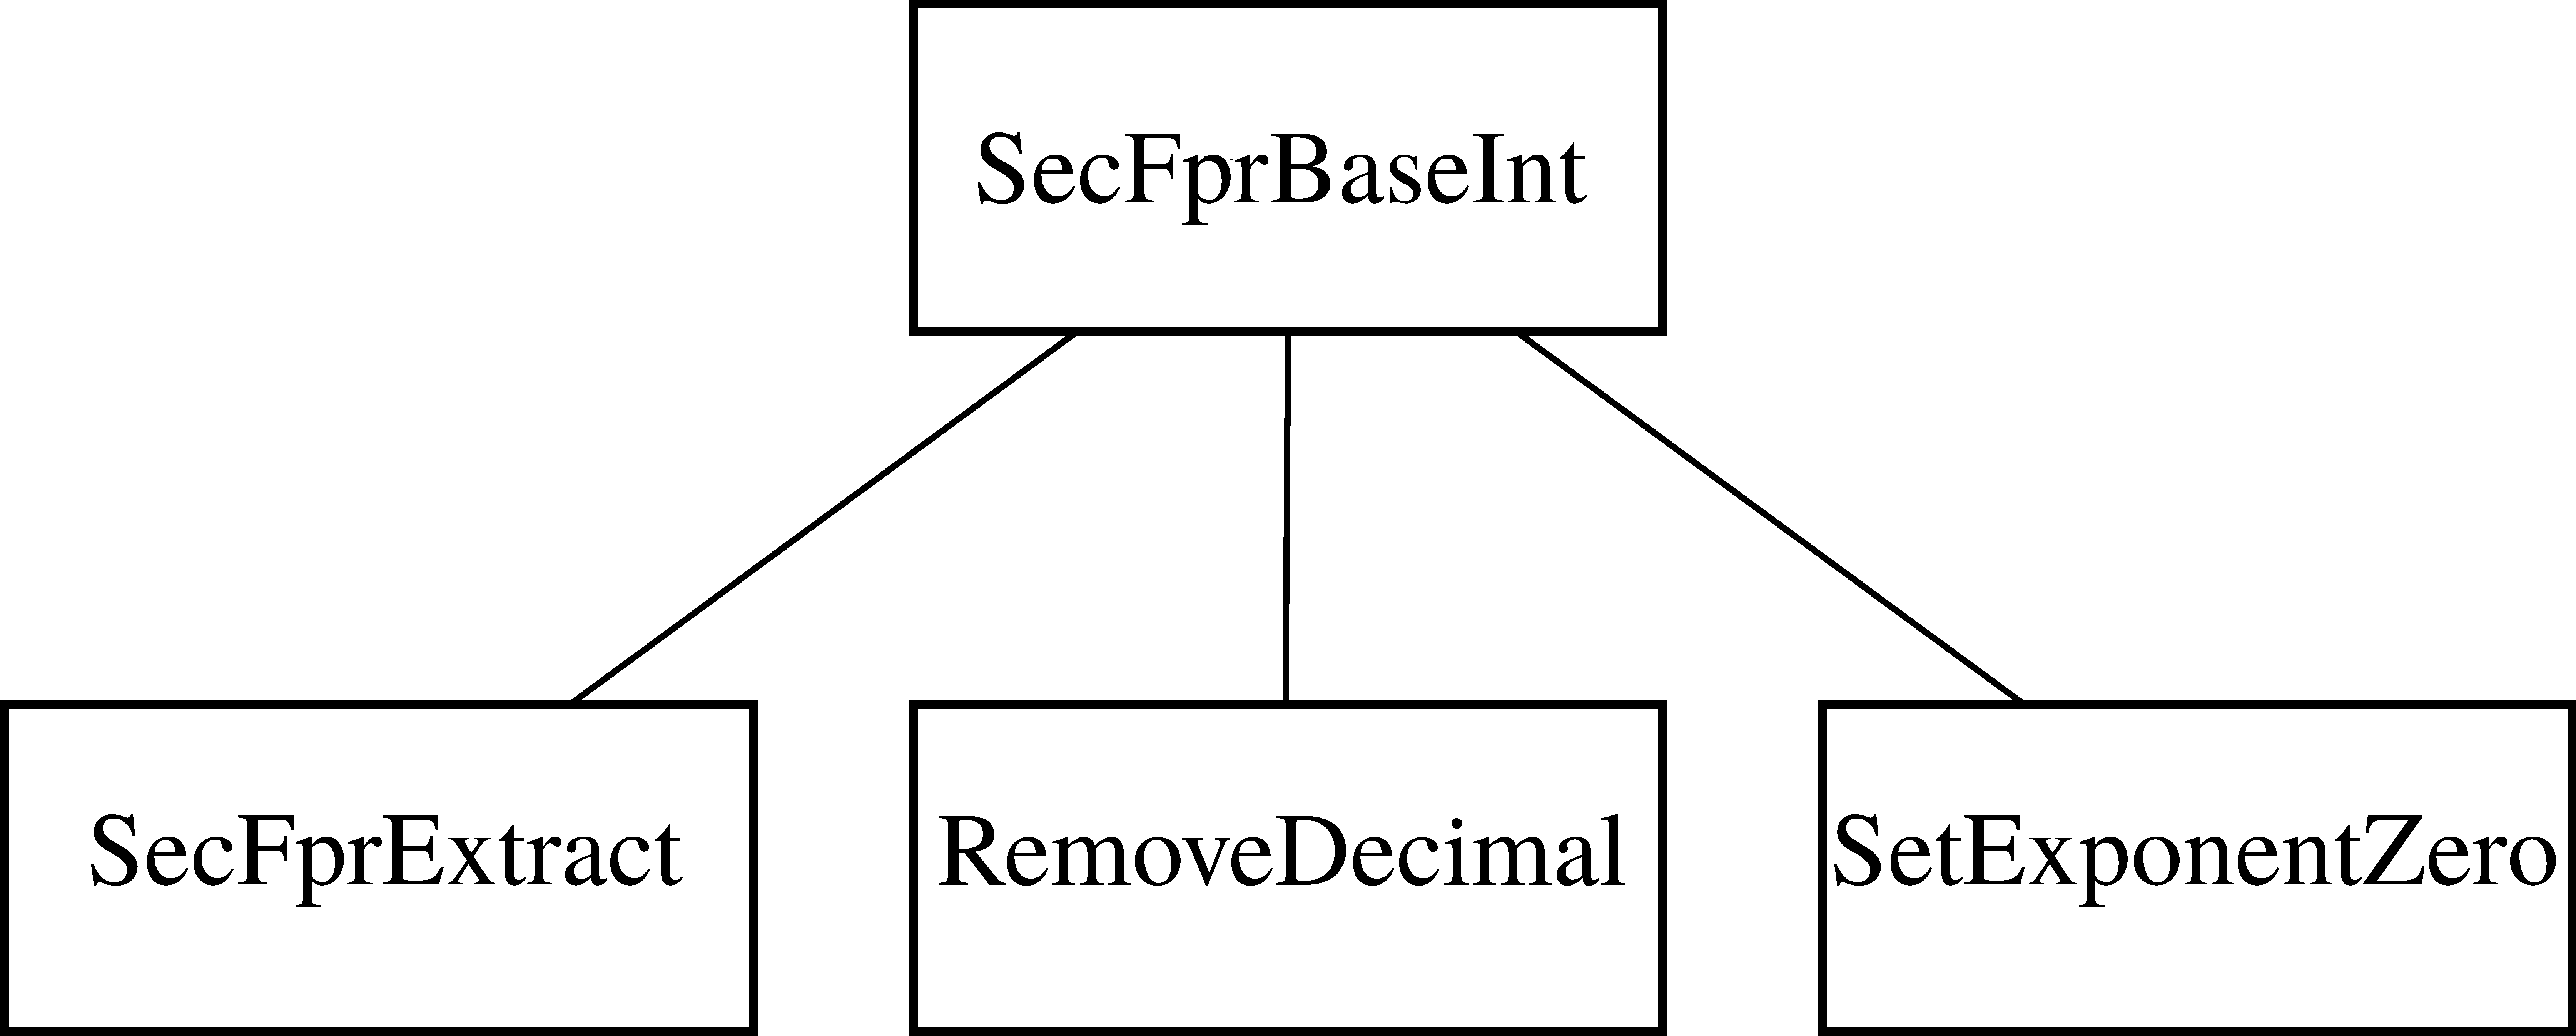
\includegraphics[width=0.5\textwidth]{figure/secpfrhierarchie.pdf}
      \label{fig:hierar}
      \caption{SecFprBaseInt and its gadgets}
  \end{figure}

  In this subsection, suppose $f$ = floor. We will first present the main structure and then present the gadgets. Gadgets from trunc and round function can be found in annexe (the little differences between gadgets will be explain too):
  \begin{itemize}%[label = $\bullet$]
      \item SetFprExtract;
      \item RemoveDecimal$_\text{trunc}$ and SetExponentZero$_\text{trunc}$;
      \item RemoveDecimal$_\text{round}$ and SetExponentZero$_\text{round}$.
  \end{itemize}
  The particularity of our shift method for calculating floor function is that it requires the gadgets proposed by Chen and Chen \cite{Chen_Chen_2024}. So by proposing this method, we are extending their work to mask the Gaussian sampler by using only the gadgets of their creation.
  By way of summary, we propose a table showing the functions used to create our gadgets and the sources from which they come.

  \begin{figure}[!ht]
      \begin{center}
          \begin{tabular}{C{2.5 cm} || C{6 cm} C{1.2cm} C{2cm}}
            \toprule
             \textbf{Algorithm} & \textbf{Description} & \textbf{Security} & \textbf{Reference}\\
              \midrule
               SecAnd   & AND of Boolean shares             & $t$-SNI &  \cite{ishai2003private}, \cite{barthe2016strong}\\
               SecAdd         & Addition of Boolean shares        & $t$-SNI&  \cite{coron2015conversion}, \cite{barthe2018masking}\\
               A2B            & Arithmetic to Boolean conversion  & $t$-SNI& \cite{schneider2019efficiently}\\
               B2A            & Boolean to Arithmetic conversion  & $t$-SNI&  \cite{bettale2018improved}\\
               RefreshMasks   & $t$-NI refresh of masks           & $t$-NI&  \cite{barthe2016strong}, \cite{bettale2018improved}\\
               Refresh        & $t$-SNI refresh of masks          & $t$-SNI& \cite{barthe2016strong}\\
               SecOr          & OR of Boolean shares              & $t$-SNI&  \cite{Chen_Chen_2024}\\
               SecNonZero     & NonZero check of shares           & $t$-SNI&  \cite{Chen_Chen_2024}\\
               SecFprUrsh     & Right-shift keeping sticky bit updated  & $t$-SNI&  \cite{Chen_Chen_2024}\\
               SecFprNorm64   & Normalization to $[2^{63},2^{64})$ & $t$-NI& \cite{Chen_Chen_2024}\\
              \bottomrule
          \end{tabular}
      \end{center}
  \end{figure}

  
    \subsubsection{SecFprBaseInt$_\text{f}$ -- \autoref{algo:SecFprBaseInt}}
    We present a global structure for all three functions f = floor/round/truncate.
    \begin{algorithm}[H]
      \caption{SecFprBaseInt$_\text{f}$(x)}
      \label{algo:SecFprBaseInt}
      \KwData{64-bit boolean shares $(x_i)_{1\leq i \leq n}$ for value x }%\\
      %A function f : floor, round or trunc.}
      \KwResult{64-bit boolean shares $(y_i)_{1\leq i \leq n}$ for mantissa value y = f(x).} 
      $((my_i), (ey_i), (sy_i)) \leftarrow$ SecFprExtract($(x_i)$)\;%\tcp*{extract mantissa, exponent and sign}
      $(cx_i) \leftarrow (ey_i)$\;
      $cx_1 \leftarrow ey_1 - \text{Zero}_f$\;%\tcp*{$\text{Zero}_f$ = 1023 for floor }%and trunc, $\text{Zero}_f$ = 1022 for round}
      $(c_i) \leftarrow$ A2B($(cx_i^{(16)})$)\; 
      Refresh($(cx_i)$)\;
      $(my_i) \leftarrow$ SecAnd($(my_i), (\neg(-c_i))$)\;%\tcp*{if c = 0,  my = mx and if c = 1, my = 0 }
      $(my_i), (ey_i), (Rnd_i) \leftarrow$ RemoveDecimal$_f((my_i), (ey_i), (sy_i), (cx_i)$)\;% \tcp*{depends on f}
      $(my_i), (ey_i) \leftarrow$ SecFprNorm64($(my_i),(ey_i)$)\;
      $(my_i) \leftarrow (my_i >> 11)$\;
      $(my_i) \leftarrow$ $(my_i^{[52:1]}) $\;
      $ey_1 \leftarrow ey_1 + 11$\;
      $(ey_i), (sy_i) \leftarrow$ SetExponentZero$_f((ey_i), (\neg(-c_i)), (s_i), (Rnd_i))$\;%\tcp*{set ey at 0 if f(x)=0}
      $(y_i^{(64)}) \leftarrow (sy_i) $\;
      $(y_i^{[63:53]}) \leftarrow (ey_i) $\;
      $(y_i^{[53:1]}) \leftarrow (my_i) $\;
    \Return{$(y_i)$}\;
    \end{algorithm}
    As explained in overview, these three functions can be summarised in a global structure. 
    What will differentiate the three functions will in fact be the gadgets and the Zero$_f$ parameter.
    To perform the floor function, we first extract the data from the encoding and place it in three variables $s_y, e_y$ and $m_y$, which will be linked directly to the output of the algorithm. 
    By extracting this data\footnote{Pseudo-code in appendix: SecFprExtract -- \autoref{algo:SecFprExtract }}, we carry out a few operations on the mantissa and the exponent to match the conventions of Chen's implementation.
      Indeed, the input $x$ is a 64-bit boolean share, consequently we'll have to transform the exponent into a 16-bit arithmetic share by performing a boolean to arithmetic conversion.
      Another important thing to add is the bit implicit in the mantissa. 
      This bit which is not present in the $x$ information, in order to save one bit and gain in precision, is nevertheless very important.
      In particular, it enables us to normalise our shares correctly.
      Once these changes have been made, we can start working on the exponent.

      Without any surprise, the first step consists of checking whether the result is an obvious zero or not.
      To do so, we compare $e_y$ and Zero$_f$ -- which is the correponding exponent to  $1=2^0$ -- by calcultating $c_x = e_y - \text{Zero}_f$.
      If $cx$ is negative, $\mid x \mid <1$ and all decimals can be removed by putting $my = 0$.
      We just need to be carefull at the end of the algorithm because of some particular cases\footnote{For example, if $-1<x<0$, we need to return encoding -1, not zero.}.
      This step without taking care of particular case corresponds in reality to the truncature.
      Otherwise, the $m_y$ mantissa will remain unchanged to be adjusted during the next steps.

      A mathematical explanation of Zero$_f$'s choice can be summurize in a few simple calculus.
      In case $f$ = floor or trunc, Zero$_f = 1023$.
      Indeed if $e_y -1023 <0$, $$2^{e_x-1023} \times (1+m_x\times 2^{-52})\quad\leq \quad 2^{-1} \times (1+m_x\times 2^{-52}) \quad< \quad 1$$ 
      We remark a difference for $f$ = round.
      The main reason of this difference is that we want to avoid to reject the case where the binary decomposition of $x$ contains a $1$ at indices $2^{-1} = 0.5$, 
      since we will no longer be able to round off the final result.
      This justify the choice of  Zero$_f =1022$ for rounding function.
      This time, if $e_y -1022 <0$: 
      $$2^{e_x-1023} \times (1+m_x\times 2^{-52})\quad\leq \quad 2^{-2} \times (1+m_x\times 2^{-52}) \quad< \quad 0.5$$ 
      
      To sum up, after the first step, only $my$ can change. The two values it can take are $my$ it-self (no changes) or $0$.
      The second step removes the decimals by shifting them to the right, using RemoveDecimal -- \autoref{algo:RemoveDecimal_floor}. 
      As this algorithm does not normalise the mantissa, we then apply the SecFprNorm64 function, !!!!!!!! followed by a refresh (SecFprNorm64 is a $t$-NI gadgets) and !!!!!!!!!!! a computation of shifted $my$ and $ey$ to set the mantissa back to bits $[52:1]$ and update $ey$.
      Finally, the last step in the algorithm, before reformatting the initial encoding, is to apply the specific encoding of "0" if this is the result to be returned.
      To do this, we apply the SetExponentZero$_f$ function -- \autoref{algo:SetExponentZero_floor}. 
      \begin{algorithm}
          \caption{RemoveDecimal$_{\text{floor}}((my_i), (ey_i), (sy_i), (cx_i))$}
          \label{algo:RemoveDecimal_floor}
          \KwData{64-bit boolean shares $(my_i)_{1\leq i \leq n}$ for mantissa value my; \\
          16-bit arithmetic shares $(ey_i)_{1\leq i \leq n}$ for exponent value ey; \\
          1-bit boolean shares $(sy_i)_{1\leq i \leq n}$ for sign value sy\\
          16-bit arithmetic shares $(cx_i)_{1\leq i \leq n}$ for value cx = ex-2013.}
          \KwResult{64-bit boolean shares $(my_i)_{1\leq i \leq n}$ for mantissa value $my >> (52 - cx)$; \\
                    16-bit arithmetic shares $(ey_i)_{1\leq i \leq n}$ for exponent value $ey +(52 - cx)$;} 
          $cx_1 \leftarrow cx_1 - 52$\;%\tcp*{check if 0$\leq$c$<$51}
          $(c_i) \leftarrow$ A2B($(cx_i)$)\;
          $(cp_i) \leftarrow (c_i^{(16)})$\;
          $(cp_i) \leftarrow$ SecNonZero($cp_i$)\;
          $(c'_i) \leftarrow (- cp_i)$\;%\tcp*{if cp = 0 cx = 0. if not cx = cx }
          $(c_i) \leftarrow$ SecAnd($(c_i), (c'_i)$)\;
          $(cx_i) \leftarrow$ B2A($(c_i)$)\;
          $(cd_i) \leftarrow (-cx_i)$\;
          $(my_i), (rot_i) \leftarrow$ SecFprUrsh$_f$($(my_i), (cd_i)$)\;%\tcp*{$my >> 52 - cx$ and $rot = my^{[52-cx:1]}$}
          $(b_i) \leftarrow$ SecNonZero($(rot_i)$)\;%\tcp*{if $b=0$, $x \in \mathbb{N}$, else $x\in \mathbb{R}/\mathbb{N}$ }
          $(cp_i) \leftarrow$ SecAnd($(cp_i), (sy_i)$)\; 
          $(cp_i) \leftarrow$ SecAnd($(cp_i), (b_i)$)\; 
          $(my_i)\leftarrow$ SecAdd($(my_i), (cp_i)$)\;%\tcp*{add 1 only if $s = 1$ and if $x \in \mathbb{R}/\mathbb{N}$}
          $(ey_i) \leftarrow (ey_i + cd_i)$\; 
        \Return{(Refresh$(my_i)$, Refresh$(ey_i))$}\;
        \end{algorithm}
  \subsubsection{RemoveDecimal$_\text{floor}$ -- \autoref{algo:RemoveDecimal_floor}}
  As we explained at the beginning of this section, we need to remove the decimals from the input number.
  After checking a first result, the mantissa is equal to 0, if $e-\text{Zero}_f<0$, or has remained unchanged.
  This leaves us with the case where a shift is needed. To do so, we write $cx = e - 1023$ as the shift to be performed.
  The case where $cx<0$ has already been treaten by modifying (or not) the mantissa, whatever shift is made, we would have $0>>cx = 0$.
  If $cx=\geq52$, $x$ is already in the correct form. In fact, we have : 
  $$\mid (-1)^s \times 2^{cx} \times(1+m\times 2^{-52})\mid \quad \geq \quad 2^{52} \times(1+m\times 2^{-52})\quad = \quad2^{52} + m \in \mathbb{N}$$
  To avoid removing information if it isn't needed, we replace $cx$ by $0$.
  Be careful if we want to round a number : it's important to compare $cx$ to $53$ instead of $52$. The reason is that we first subtract to $ey$ $1022$ instead of $1023$ when we were checking is the result was 0 or not. So here we need to add 1.
  If $0\leq e_y - 1023 \leq 51$, we need to modify the mantissa to remove -- if necessary-- the decimals.
  Remarks that even in this case, the mantissa can be in the good format. For example if $x = 5$, we have $0\leq e_y-1023 = 1025-1023 = 2 \leq 51$ and $x$ is an integer.
  
  After verifying is $x$ is or isn't a "big" number, i.e. without decimal in its representation, we can shift\footnote{
  In pseudo-code the subtraction is implicite due to the format of a masked value.} $my$ by $cd=52-cx$ by applying a modified \footnote{If
  we want to use Chen's algorithm, it's possible. We just need to compute one shift less then described in our algorithm and then compute an extra shift manually. The disadvantges of using it, is that you need to check if $cx$ is different from $0$ 
  -- to not compute a shift if it isn't needed -- and the cost of computing the sticky bit.} SecFprUrsh$_f$ -- \autoref{algo:SecFprUrsh}: 
  we don't want to keep the sticky bit, so we just removed this part.
  We had an extra output, returning the part we removed.
  Shift a value is a good thing, but that's not exactly the floor function. After this step we just have the truncature.
  When $x$ positive there's no problem at all, floor function is equal to truncature. But when $x$ is negative there is one. It cames from floor properties. Indeed if $x<0$ : 
  \begin{equation}
      \label{eq:floorneg}
      \text{floor}(-x)  = \Bigg\{ \begin{array}{cc}
          \text{trunc}(-x) &  \text{if } x\in\mathbb{N}\\
          \text{trunc}(-x) -1 &  \text{if } x\in\mathbb{R}/\mathbb{N}
       \end{array}
  \end{equation}

  On one hand, checking if $x$ is negative is quite easy : we just have to take a look at if $sy$ is equal to 1.
  On the other hand, checking that $x$ is an integer is trickier. This is where the second modification to SecFprUrsh$_f$ comes in handy. As this function performs a rotation, the bit information is retained until a mask is applied to calculate the shift. 
  We therefore decided to invert the mask in order to retain the suppressed information. If this information has zero Hamming weight
  then $x$ is an integer. We can then use the SecNonZero gadget on this information, which will return $0$ if $x$ is an integer, and 1 if not.
  We denote this result $b=$ SecNonZero(($my_i^{[52 - c_x:1]}$)). 
  In the following truth table (\autoref{figure:flooradjust}) if the result $cp = $ $s$ AND $b$ is $1$, the mantissa must be changed.
  \begin{figure}
      \begin{center}
          \begin{tabular}{C{0.5cm} C{0.5cm} || C{3 cm} L{3cm}}
              \hline $sy$ & $b$ &$cp$ = $sy$ AND $b$ & Interpretation\\
              \hline 
              0 & $b$ & 0 & Positive number\\
              1 & 0  & 0 & $x$ is an integer\\
              1 & 1  & 1 & Negative real\\ \hline
          \end{tabular}
      \end{center}
      \caption{Do we need to subtract $s$: Truth table}
      \label{figure:flooradjust}
  \end{figure}
  Another question is now : how to subtract $s$ from the mantissa if the mantissa is always positive? 
  The sign of $x$ is only define by $sy$, so $\mid x\mid = 2^{ey-1023}\times(1 + my\times 2^{-52})$.
  We already know that if $x$ is positive or an integer,$my = my \pm 0 = my \pm cp$.
  Now let's focus on $x$ a non integer negative number. Let $x$ be a positive real, from \autoref{eq:floorneg}, we can write :
  \begin{equation}\label{eq:floorabs}
      my =\: \mid \text{floor}(-x)\mid \:=\: \mid \text{trunc}(-x) - 1\mid
  \end{equation}
  By using $\mid \text{trunc}(-x) \mid \:=\: \mid -\text{trunc}(x)\mid \:$, we can transform \autoref{eq:floorabs} :
  \begin{equation}\label{eq:floorabs2}
      my =\: \mid \text{floor}(-x)\mid \:=\: \mid -\text{trunc}(x) - 1\mid \:=\: \mid \text{trunc}(x) + 1\mid \:= my + cp
  \end{equation}
  \begin{algorithm}
    \caption{SecFprUrsh$_{\text{floor}}((my_i), (cx_i))$}
    \label{algo:SecFprUrsh}
    \KwData{ 6-bit arithmetic shares $(cx_i)_{1\leq i \leq n}$ for value cx; \\
    64-bit boolean shares $(my_i)_{1\leq i \leq n}$ for sign value $my$.}
    \KwResult{64-bit boolean shares $(my'_i)_{1\leq i \leq n}$ for value $my>>cx$\\
    64-bit boolean shares $(rot_i)_{1\leq i \leq n}$ for value $my^{[cx : 1]}$.} 
      $(m_i)_{1\leq i \leq n} \leftarrow ((1<<63), 0, \cdots, 0)$\;
      \For{\texttt{i from 1 to n}}{
        Right-Rotate $(my_i)$ by $cx_j$\;
        $(my_i) \leftarrow$ RefreshMasks($(my_i)$)\;
        Right-Rotate $(m_i)$ by $cx_j$\;
        $(m_i) \leftarrow$ RefreshMasks($(m_i)$)\;
      }
      $len \leftarrow 1$\;
      \While{$len\leq 32$}{
        $(m_i) \leftarrow (m_i \oplus (m_i>>len))$\;
        $len \leftarrow len<<1$\;
      }
      $(my'_i) \leftarrow$ SecAnd($(my_i), (m_i)$)\;
      $(m_i) \leftarrow (\neg(m_i))$\;
      $(rot_i) \leftarrow$ SecAnd($(my_i), (m_i)$)\;
  \Return{$((my'_i), (rot_i))$}\;
  \end{algorithm}
  From this, we only have to compute a secure addition between $cp$ and $my$.
  The last step of this algorithm is to add the shift $cd$ to $ey$ to keep this data update.
  \begin{algorithm}
      \caption{SetExponentZero$_{\text{floor}}((ey_i), (sy_i), (b_i))$}
      \label{algo:SetExponentZero_floor}
      \KwData{ 16-bit arithmetic shares $(ey_i)_{1\leq i \leq n}$ for exponent value ey; \\
      1-bit boolean shares $(sy_i)_{1\leq i \leq n}$ for sign value sy\\
      64-bit boolean shares $(b_i)_{1\leq i \leq n}$.}
      \KwResult{16-bit boolean shares $(ey_i)_{1\leq i \leq n}$ for exponent value $ey +(52 - cx)$;\\
                1-bit boolean shares $(sy_i)_{1\leq i \leq n}$ for sign value.} 
      
        $(ey_i) \leftarrow$ A2B($(ey_i)$)\;
        $(b'_i) \leftarrow (-sy_i)$\;
        $(b'_i) \leftarrow$ SecOr($(b'_i), (b_i)$)\;
        $(ey_i) \leftarrow$ SecAnd($(ey_i, b'_i)$)\;
        $(sy_i) \leftarrow$ SecAnd($(sy_i, b'_i)$)\;
    
    \Return{$((ey_i), (sy_i))$}\;
    \end{algorithm}
  \subsubsection{SetExponentZero$_\text{floor}$ -- \autoref{algo:SetExponentZero_floor}}

  This last function, which is useful in the algorithm, uses the data collected throughout the calculations of the whole algorithm to modify $ey$ and $sy$ if the expected result is 0.
    The encoding of $0$ is special because it is encoded by itself. It must therefore be possible to update $ey$ and $sy$ if necessary. 
    For the floor function, we need the $sy$ sign bit and the $b$ mantissa zero condition.
    The desired result is zero only if $\mid x \mid <1$ and $sy=0$. Recall that if $sy=1$ and $\mid x \mid <1$, floor($x)=-1$. 
    Minus 1's encoding is $sy = 1$, $ey = 1023$ and $my = 0$.

    \begin{figure}
      \begin{center}
          \begin{tabular}{C{1.2cm} C{1.2cm} || C{2 cm} C{7.5cm}}
              \hline $-sy$ & $b$ &$-sy$ OR $b$ & Interpretation\\
              \hline 
              $0\cdots0$ & $0\cdots0$ & $0\cdots0$ & "Small" positive number : $ey = 0$ and $sy = 0$  \\
              $1\cdots1$ & $0\cdots0$ & $1\cdots1$ & "Small" negative number : $ey = 1023$ and $sy = 1$\\ 
              $-sy$ & $1\cdots1$ & $01\cdots1$ & Non zero number : $ey = ey$ and $sy=sy$\\\hline
          \end{tabular}
      \end{center}
      \caption{Encoding 0, minus 1 or others: Truth table}
      \label{figure:flooradjust2}
  \end{figure}
%
% ---- Bibliography ----
%
% BibTeX users should specify bibliography style 'splncs04'.
% References will then be sorted and formatted in the correct style.
%
 \bibliographystyle{splncs04}
 \bibliography{falcon}

\end{document}
